
%%%%%%%%%%%%%%%%%%%%%%%%%%%%%%%%%%%%%%%%%%%%%%%%%%%%%%%%%%%%%%%%%%%%%%%%%%%%%%%
%
% Nicole's Thesis, IIT 2018
%
%%%%%%%%%%%%%%%%%%%%%%%%%%%%%%%%%%%%%%%%%%%%%%%%%%%%%%%%%%%%%%%%%%%%%%%%%%%%%%%
\documentclass{iitthesis}

% Document Options:
%
% Note if you want to save paper when printing drafts,
% replace the above line by
%
%   \documentclass[draft]{iitthesis}
%
% See Help file for more about options.

\usepackage{graphicx}    % This package is used for Figures
\usepackage{rotating}           % This package is used for landscape mode.
\usepackage{epsfig}
\usepackage{subfigure}          % These two packages, epsfig and subfigure, are used for creating subplots.
\usepackage{siunitx}
\usepackage{url}
\usepackage{tikz}
\usepackage[american]{circuitikz}
\usepackage[normalem]{ulem}
\usetikzlibrary{shapes.misc}
\usetikzlibrary{shapes,arrows,decorations.markings,shadows,positioning}

%% Only for editing process...TAKE OUT for FINAL DRAFT
\usepackage{graphicx,xcolor,enumitem}
\newcommand{\lsnote}[1]{\textsf{{\color{violet}{ LS note:}   #1 }}}
\newcommand{\nrnote}[1]{\textsf{{\color{blue}{ NN note:}   #1 }}}
\newcommand{\jpnote}[1]{\textsf{{\color{green}{ JP note:}   #1 }}}
%\lsnote{\sout{ This is how you strike through text}}


\begin{document}

\title{Design for Staged Two Beam Acceleration at the Argonne Wakefield Accelerator Facility}

\author{Nicole Neveu }
\degree{Doctor of Philosophy}
\dept{Physics}
\date{May 2018}
\copyrightnoticetrue      % crate copyright page or not
%\coadvisortrue           % add co-advisor. activate it by removing % symbol to add co-advisor
\maketitle                % create title and copyright pages


\prelimpages         % Settings of preliminary pages are done with \prelimpages command

%%%  Acknowledgement %%%
\begin{acknowledgement}     % acknowledgement environment, this is optional
	\par  Family, Lalo, Linda, John, AWA group, Jeff
	%\input{ackno.tex} % you need a separate acknowledgement.tex file to include it.
\end{acknowledgement}

% Table of Contents
\tableofcontents
\clearpage

% List of Tables
\listoftables
\clearpage

%List of Figures
\listoffigures
\clearpage

%List of Symbols(optional)

\listofsymbols
\SymbolDefinition{$c$}{Speed of Light}
\SymbolDefinition{$\epsilon$}{Dielectric Permittivity}
\SymbolDefinition{$\epsilon$}{6D Phase Space Emittance}
\SymbolDefinition{$\gamma$}{Relativistic Kinetic Energy}

\clearpage

%%% Abstract %%%
\begin{abstract}           % abstract environment, this is optional
	\par Staged two beam acceleration using dielectric structures has yet to 
	be achieved anywhere in the world. In this thesis, I discuss the beam 
	line design and simulation, followed by experimental results of a 
	beam line with the potential for dielectric TBA.   
\end{abstract}

\textpages     % Settings of text-pages are done with \textpages command

\Chapter{INTRODUCTION}
%%%%%%%%%%%%%%%%%%%%%%%%%%%%%%%%%%%%%%%%%%%%%%%%%%%%%%%%%%%%%%%%%%%%%%%%%%%%%%%%%%%%%%%%%%%%
%%%%%%%%%%%%%%%%%%%%%%%%%%%%%%%%%%%%%%%%%%%%%%%%%%%%%%%%%%%%%%%%%%%%%%%%%%%%%%%%%%%%%%%%%%%%
\Section{Motivation} \label{sec:motivation}
%%%%%%%%%%%%%%%%%%%%%%%%%%%%%%%%%%%%%%%%%%%%%%%%%%%%%%%%%%%%%%%%%%%%%%%%%%%%%%%%%%%%%%%%%%%%
%%%%%%%%%%%%%%%%%%%%%%%%%%%%%%%%%%%%%%%%%%%%%%%%%%%%%%%%%%%%%%%%%%%%%%%%%%%%%%%%%%%%%%%%%%%%
A new generation of accelerators dedicated to High Energy Physics
(HEP), would likely be of the TeV scale. Reduction in the size and cost
of such machines is key to their feasibility, and can be accomplished
through accelerator technology R\&D. Investigation into a 
high gradient candidate for future HEP machines is an active research area
at the Argonne Wakefield Accelerator (AWA) facility. A
short pulse, two-beam acceleration (TBA) scheme using 
wakefield power extractors, and accelerating structures made 
of metallic materials was demonstrated~\cite{recent-tba}. 
A goal of the AWA group is to demonstrate fully staged TBA, 
achieving a gradient of 250 MV/m. If successful, this would
be the only facility in the world capable of such gradients used for
acceleration of a beam.

TBA requires a drive beam to pass through a decelerating structure and
loss of energy through wakefield generation. The electromagnetic wake
is coupled from the decelerator into an accelerating structure, where
the electric field is used to accelerate a second beam. In order to have equivalent power 
generation for each stage, two complete and separate beamlines 
operating synchronously with each other are required.  
The wakefield structures can be metallic or dielectric. Dielectric
structures, having no irises, are simple to manufacture and have demonstrated
high gradient capability at \SI{100}{MV/m} \cite{WeiPaper}. 

The Compact Linear Collider (CLIC) collaboration, proposes a similar TBA scheme with
a \SI{240}{ns} pulse design. This limits the acceleration gradient
to roughly \SI{150}{MV/m} at room temperature due to rf breakdown \cite{CLICdesignReport}.
Higher gradients could be reached when driven by a very short drive
beam pulse, such as the 20ns pulse length proposed by AWA \cite{WeiPaper}. 
\nrnote{Understand and explain why short pulse can give higher gradients. 
Because higher peak power is tolerable, but average power stays the same?}
While the two groups vary on approach, they agree that TBA would 
require less infrastructure when constructing a linear TeV scale machine, 
versus the cost of more conventional technology. 
For example, a case study was done comparing the infrastructure 
needed when using traditional \SI{50}{MW} klystron sources.
It would take roughly 35,000 klystrons to construct a linear machine to deliver the same 
\SI{9.2}{TW} power as in the CLIC design specification in CLIC reports \cite{CLICdesignReport}. 
In comparison to CLIC's 48 km projected machine length needed to reach \SI{3}{TeV}, the Next Linear
Collider (NLC) collaboration projected a machine length of \SI{26}{km} using X-band klystrons,
only to reach an energy of \SI{1}{TeV}. %\cite{NLC}. 
\lsnote{The text below is not well developed.  I guess since it is in this paragraph, you are trying to explain the statement that less infrastructure is required.  First, you don't say anything specifically about using an accelerator beam rather than a klystron - how does that save on equipment and space?  It is also confusing that you start by saying the power to the witness beam is conventional, abut then say there is a difference in infrastructure with nothing between  about why.}
The power supplied to the witness beam in TBA is similar to
power provided by traditional accelerator technology. 
The key difference is the amount of infrastructure and cost 
needed to transport the power. Theoretically, TBA can deliver
the same amount of power as conventional methods with less 
infrastructure, and therefore lower cost, in the case of a high energy machine. 

\lsnote{This next section of text should be a summary of what was done for your thesis, what the results were, and why they were important. Perhaps mapping them to the corresponding sections of your thesis.  The AWA facility and following sections should probably be in the next chapter.  You probably can't write these paragraphs until finishing your work.}

Before a detailed understanding of the power and infrastructure trade offs 
can be obtained, the feasibility of staged TBA must be be demonstrated as viable, 
as no high energy machine can be built without staging.
Staging is the ability to use two successive accelerating modules to synchronously accelerate 
the same particle bunch. While simple in principle, the difficulties 
in achieving staging should not be underestimated. 
Demonstration of staging proves that a TBA scheme can be scaled to high energies, and whether it is 
feasible to use such methods. Single stage TBA, and staging 
in a simplified scheme have been demonstrated at the AWA in 2016.
\nrnote{Not any more? - Demonstration of the full-scale dielectric staging scheme is the 
	subject of this thesis.} 
Desing and partial testing of a full-scale staging scheme is the 
subject of this thesis. The branched drive beam line was designed and 
simulated. 
Optimization of the bunch train timing took place, \nrnote{not? - the two 
	beam lines were synchronized and experimental measurements 
	of staged TBA were taken. }
Experimental results and comparison to simulations, along 
with the following beam dynamics analysis is shown here.

%%%%%%%%%%%%%%%%%%%%%%%%%%%%%%%%%%%%%%%%%%%%%%%%%%%%%%%%%%%%%%%%%%%%%%%%%%%%%%%%%%%%%%%%%%%%
%%%%%%%%%%%%%%%%%%%%%%%%%%%%%%%%%%%%%%%%%%%%%%%%%%%%%%%%%%%%%%%%%%%%%%%%%%%%%%%%%%%%%%%%%%%%
\Section{Argonne Wakefield Accelerator Facility} \label{sec:facility}
%%%%%%%%%%%%%%%%%%%%%%%%%%%%%%%%%%%%%%%%%%%%%%%%%%%%%%%%%%%%%%%%%%%%%%%%%%%%%%%%%%%%%%%%%%%%
%%%%%%%%%%%%%%%%%%%%%%%%%%%%%%%%%%%%%%%%%%%%%%%%%%%%%%%%%%%%%%%%%%%%%%%%%%%%%%%%%%%%%%%%%%%%
The AWA facility houses two rf photoinjector electron guns operating
at \SI{1.3}{GHz}, and three subsequent beam lines. 
Two of the beam lines are currently used for staged TBA, and the
third is used for Emittance Exchange experiments (EEX). A layout of
the facility is shown in Fig. \ref{fig:bunker}. 
\lsnote{Some more detail will be needed here, maybe just switch the order of the some of the text in the two paragraphs below.  Something like; start with saying what the beamlines are and what is in them referring to the figure, then describe their sources in more detail (RF guns and photocathodes), then talk about the laser and how it is split.}

Electron bunches in a photoinjector are created through the photoelectric effect. 
At the AWA, a pulsed UV laser is propagated through two relay lines of UV optics to either
the drive or witness gun. An in-vacuum mirror then directs the pulse to the photocathode.
Both beam lines must be operated simultaneously when the TBA experiments are run. This is accomplished by
splitting the original laser pulse into two pulses using a UV splitter on the 
ceiling of the bunker. One of the split pulses is sent (as is) to the witness beam line for one
bunch operation. The second pulse is sent to a UV multispitter table, shown in 
Fig.~\ref{fig:optics} where it is split into trains of various lengths. Eight pulses are 
used for TBA drive trains, 

The beam line located on the right side of Fig. \ref{fig:bunker} is called the
drive line. The rf photoinjector on the drive line uses a semiconducting
CsTe cathode, and is followed by a linear accelerator (linac). The
drive linac uses six copper cavities and four klystrons to accelerate the drive beam
to energies of 50-\SI{70}{MeV}. The number of bunches generated from each 
laser pulse can vary from 1, 2, 4, 6, and 8 bunches. When multiple bunches
are generated, the grouping is called a bunch train. Generation of
these variable bunch trains is accomplished by splitting the pulsed
UV laser beam before it enters the gun and hits the cathode. The splitting
takes place in a complex network of UV optics located near the drive
gun. The optics set up is called a beam splitter, or mulitsplitter,
and trains are created at a rate of 0.5, 1, or \SI{2}{Hz}. This timing is
called a pulse, or the repetition rate of the machine. A picture of
the AWA multisplitter table is shown in Fig. \ref{fig:optics}. Optimization 
of the UV optics was performed and is detailed in Section \ref{sec:uvoptics}.  

\iffalse
\begin{figure}
	\begin{center}
		%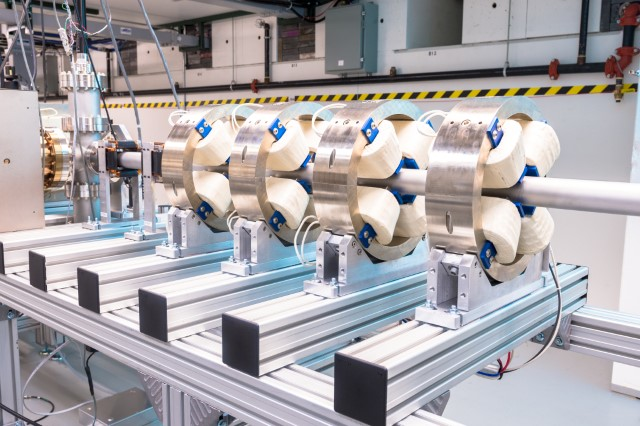
\includegraphics[width=\linewidth]{images/quads1}
		\label{fig:bunker}
	\end{center}
\end{figure}
\begin{figure}[h]
	\begin{center}
		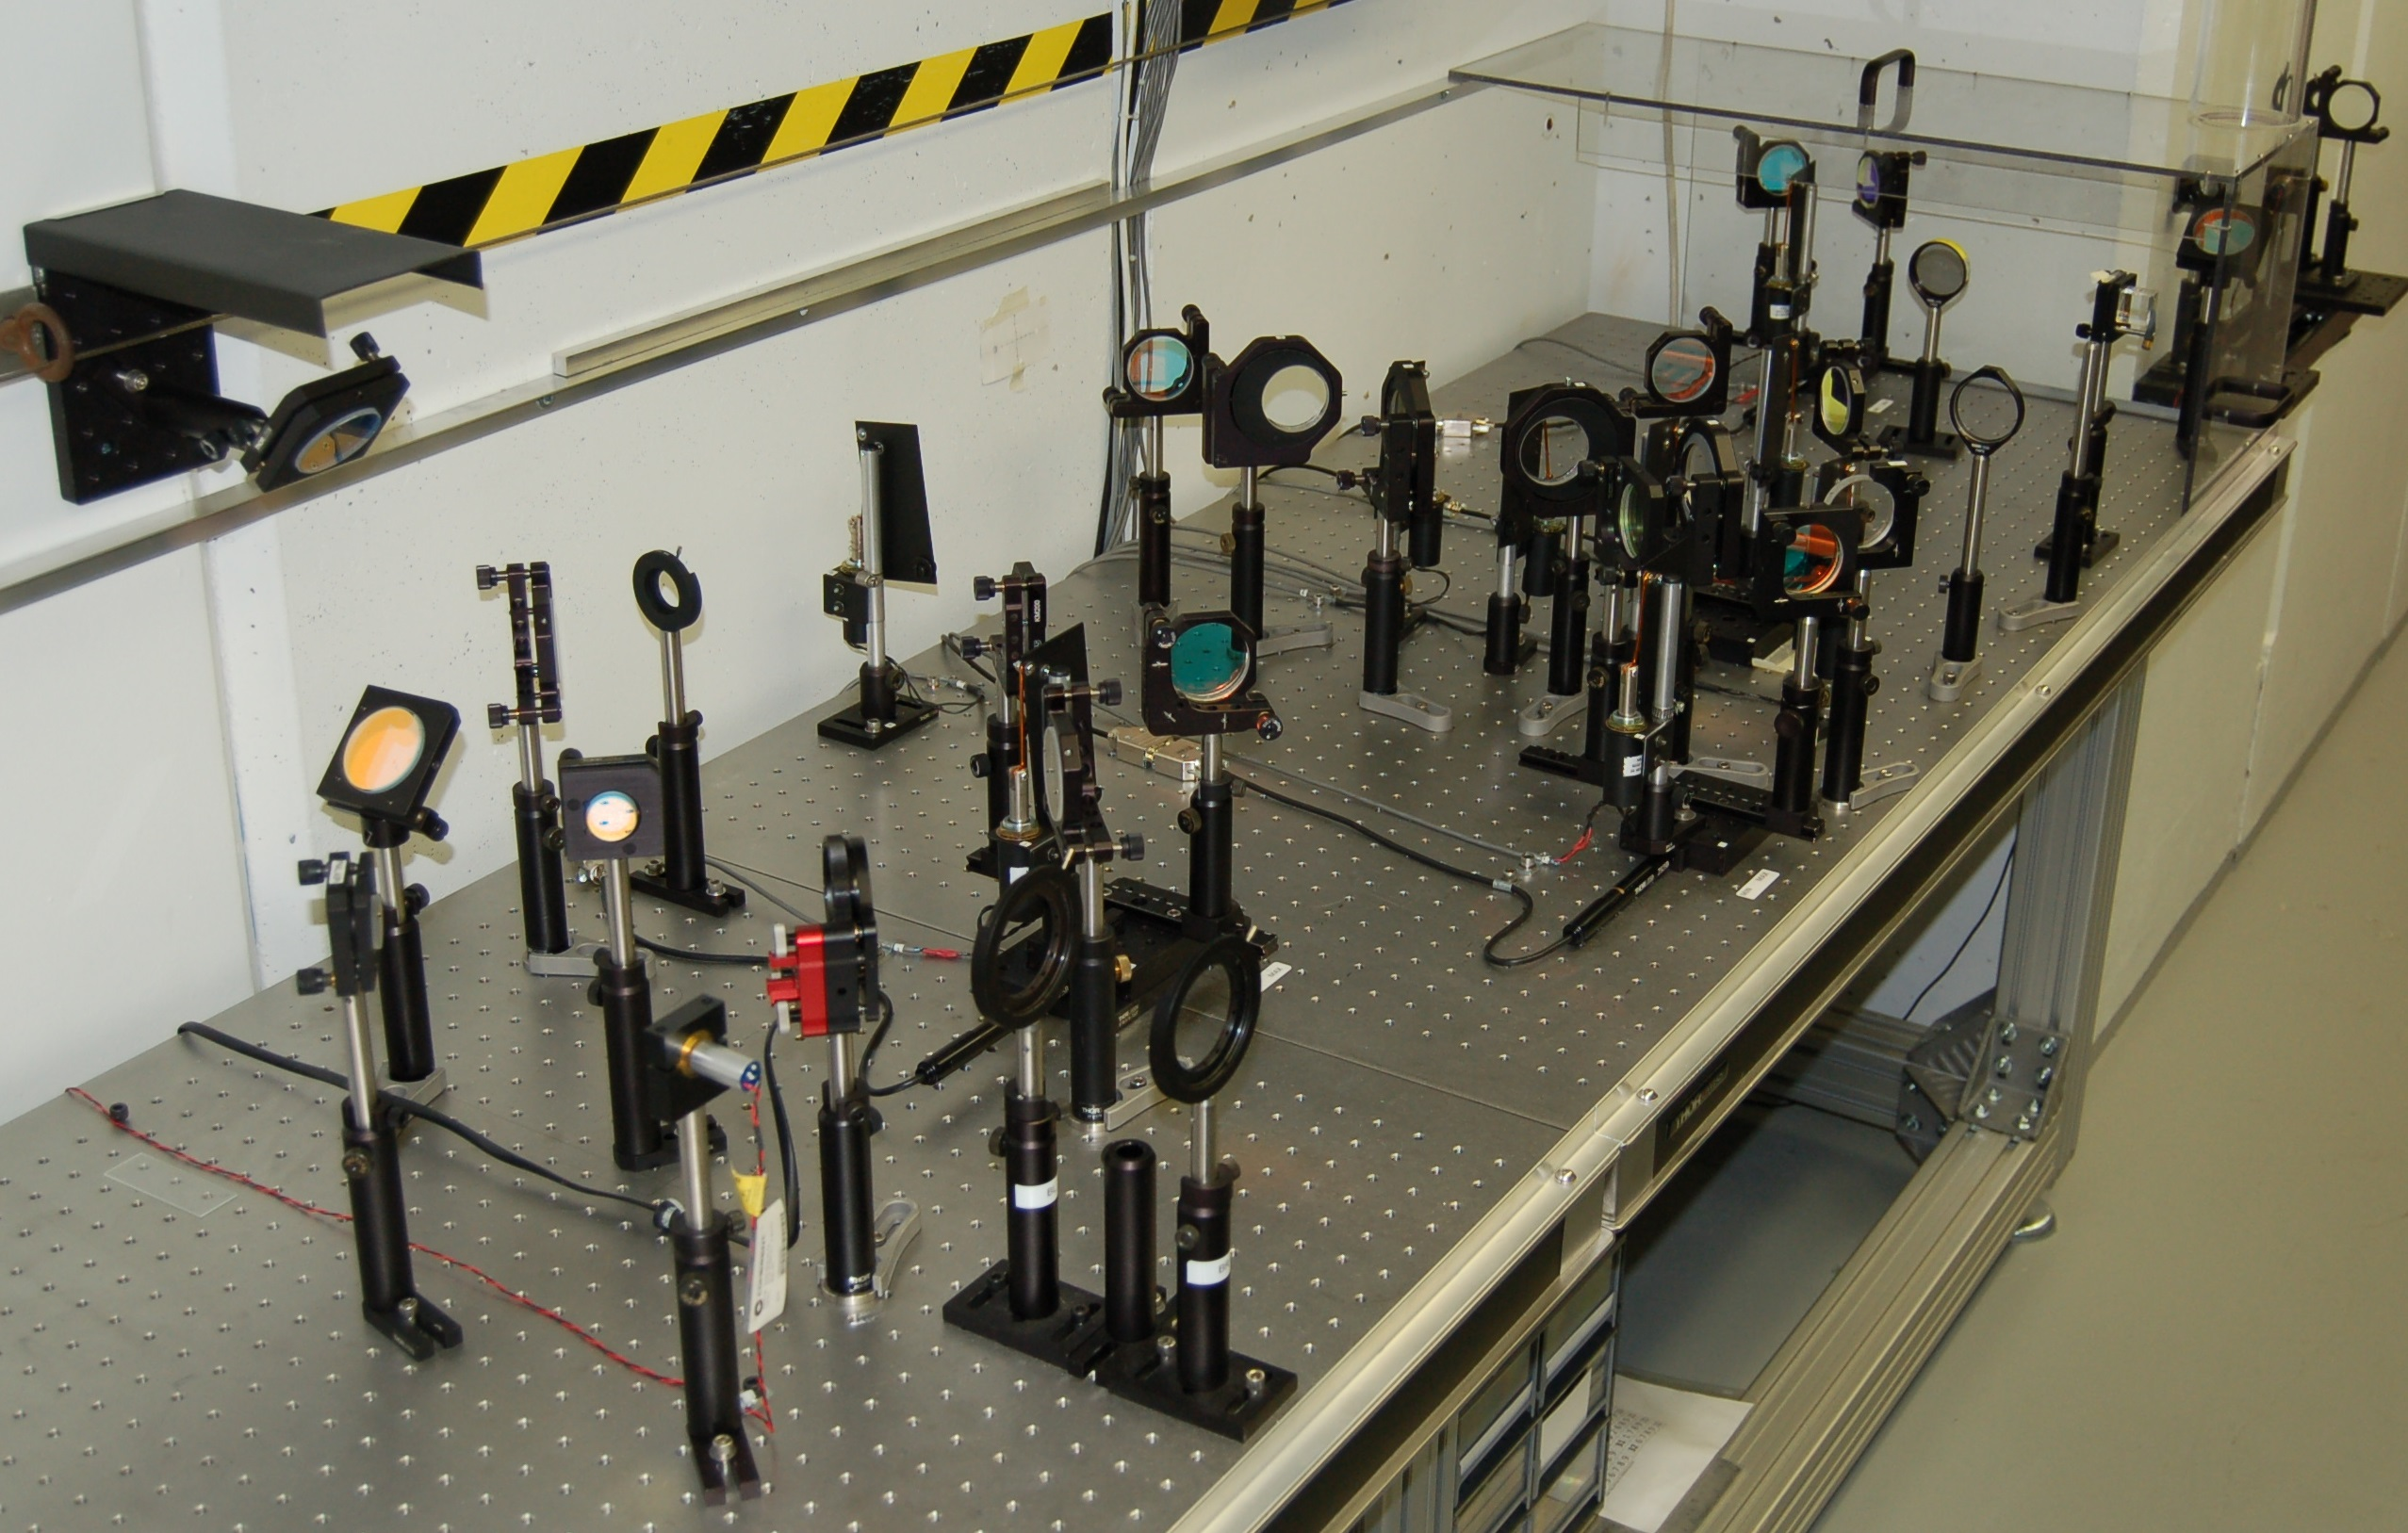
\includegraphics[width=0.5\textwidth]{images/multisplitter}\caption{UV multisplitter optics table.}
	\end{center}
	\label{fig:optics}
\end{figure}
\fi

The witness line rf photoinjector, located on the left side of Figure
1, uses a Mg cathode and the following linac consists of one copper
accelerating cavity. Prior to the multisplitter table, shown in
Fig. \ref{fig:optics}, the laser pulse is split between the drive and witness side.
This set up allows only one bunch per pulse on the witness line. Also
note that the beam from the drive line travels in the opposite direction
than the beam in the witness line. 

%%%%%%%%%%%%%%%%%%%%%%%%%%%%%%%%%%%%%%%%%%%%%%%%%%%%%%%%%%%%%%%%%%%%%%%%%%%%%%%%%%%%%%%%%%%%
%%%%%%%%%%%%%%%%%%%%%%%%%%%%%%%%%%%%%%%%%%%%%%%%%%%%%%%%%%%%%%%%%%%%%%%%%%%%%%%%%%%%%%%%%%%%
\Section{Dielectric Structures}

%%%%%%%%%%%%%%%%%%%%%%%%%%%%%%%%%%%%%%%%%%%%%%%%%%%%%%%%%%%%%%%%%%%%%%%%%%%%%%%%%%%%%%%%%%%%
%%%%%%%%%%%%%%%%%%%%%%%%%%%%%%%%%%%%%%%%%%%%%%%%%%%%%%%%%%%%%%%%%%%%%%%%%%%%%%%%%%%%%%%%%%%%
\Subsection{Power Generation}

\lsnote{Somewhere you need a comprehensive description of simplified staging vesus full staging.  I am not sure it is here, but it should be before you mention simplified staging.}

Currently, all \lsnote{define PETS acronym} PETS and accelerating structures installed in the AWA's
simplified staging scheme are metallic. It has been shown that a few
key equations can demonstrate the relationship between beam parameters
and the resulting \lsnote{\sout{rf} power} generated in the decelerating cavity. This section
borrows heavily from previous work at CLIC and the AWA \cite{key-3,key-8}. 
Starting with the timing, each bunch in the drive train will generate
an rf pulse of finite length in the structure. Each bunch is separated
in time by $T_{b}$, and the \lsnote{average?} beam current can be written as $I=\frac{Q}{T_{b}}$.
\lsnote{define Q, is it the charge per bunch?} The bunches are Gaussian in the longitudinal direction, and the form
factor, $\Phi$, is used to describe\lsnote{\sout{s}} the Gaussian shape by taking
the Fourier transform of the charge distribution: 
\begin{equation}
\Phi=exp\left[\frac{-(k_{z}\sigma_{z})^{2}}{2}\right]
\end{equation}
Where $k_{z}=\frac{2\pi}{\lambda_{z}}$ is the longitudinal wave number
and $\sigma_{z}$ is the rms bunch length. \lsnote{That was confusing.  You said phi was the FT of the charge distribution, but in the equation after that it looks like the charge distribution not the FT}  Note the subscript z \lsnote{indicates \sout{refers to the characteristics of the cavity and bunch in}} the longitudinal
direction. Then using the partial differential equation that relates
the power generated by the wakefield to the change in power over time, \lsnote{I would include the equation}
the power generated by a bunch train can be written as:
\begin{equation} \label{eq:rfpower}
P_{t}(t)=\frac{\omega_{z}\,L^{2}I^{2}}{4\,v_{g}}\frac{R}{Q_{d}}\left(\frac{1-e^{-\alpha L}}{\alpha L}\right)\Phi^{2}
\end{equation}
With $I$ being the beam current as defined above, $\alpha=\frac{\omega}{2Q_{d}v_{g}}$
being the attenuation constant \cite{key-9}, R is the shunt impedance
per unit length, and $Q_{d}$ is the quality factor for the decelerating
structure. \lsnote{You didn't define L or vg} Note, the derivation of equation 4 can be found in reference
\cite{key-8}, and due to the complex geometry of metallic structures,
the value of R/Q is often calculated in electromagnetic codes such
as CST Microwave Studio. 

\lsnote{You probably were intending to do this, but this section should close out with a predicted power generation 
in the decelerating structures.  The discussion of how that depends on number of bunches in the bunch train should be here as well.}

\Subsection{Accelerating Structures}

\Section{Two Beam Acceleration}

\Section{AWA Design Requirements} \label{sec:requirements}

\lsnote{This is probably where you should have the overview of simple staging versus full staging, and a summary of what was required to go to full staging.  The title of the section should also be changed, maybe `Fully staged two beam acceleration'?}

In order to design and test the desired beam line, three technologies 
new to the AWA were investigated. These include a kicker, septum magnets, 
and non-GA optimization algorithms.

% An example for enumerate
\begin{enumerate}
	\item Kicker Design
	\item Septum Design
	\item Optimization 
\end{enumerate}

% A quotation example
% Every quota must be accompanied by a reference to the source
% in a footnote or in the Bibliography
\begin{quotation}
	test
\end{quotation}

\clearpage


\Chapter{Experimental Set Up}
Before final measurements or meaningful simulations can be done, 
a fair amount of set up and preliminary measurements 
must be made and understood. 

%%%%%%%%%%%%%%%%%%%%%%%%%%%%%%%%%%%%%%%%%%%%%%%%%%%%%%%%%%%%%%%%%%%%%%%%%%%%%%%%%%%%%%%%%%%%
%%%%%%%%%%%%%%%%%%%%%%%%%%%%%%%%%%%%%%%%%%%%%%%%%%%%%%%%%%%%%%%%%%%%%%%%%%%%%%%%%%%%%%%%%%%%
\Section{Laser Pulse Train Improvement} \label{sec:uvoptics}
%%%%%%%%%%%%%%%%%%%%%%%%%%%%%%%%%%%%%%%%%%%%%%%%%%%%%%%%%%%%%%%%%%%%%%%%%%%%%%%%%%%%%%%%%%%%
%%%%%%%%%%%%%%%%%%%%%%%%%%%%%%%%%%%%%%%%%%%%%%%%%%%%%%%%%%%%%%%%%%%%%%%%%%%%%%%%%%%%%%%%%%%%

Ideally, to extract maximum power from a series of bunches, each electron bunch should have the same amount of charge.  Improving the laser pulse train intensity distribution improves the electron bunch charge distribution; 
which  helps produce an RF power pulse that is closer to uniform. 
The generated power depends on both the charge and shape of the bunch, as shown in Eq.~\ref{eq:rfpower}. 
Several factors contribute to non-uniformity in the bunches. These include the cathode material
(i.e. slightly different QE along the surface), shot to shot noise in the laser pulse, 
distortion of laser pulses due to traveling through air, and the quality of the optics. 
The last is especially important in determining the intensity of each laser pulse in the train.  
Each splitter has a slightly different value for transmitted (T) and reflected (R) pulses. 

\Subsection{UV Optics} 
In order to generate the drive bunch trains needed for TBA, a UV laser pulse is split 
by five optical splitters into two trains of eight pulses. 
The optics set up is shown in Fig~\ref{fig:optics}. Optical delay lines (two mirrors) near each splitter 
separate pulses in space and time by extending the distance that each pulse travels. 
The length of each delay line is a multiple of the RF frequency, 1.3 GHz. 
In other words, a separation of $1\lambda=\SI{769}{ps}$ between each UV pulse is created. 
This is done to synchronize the laser pulses with the RF supplied to the gun.
In order to achieve equally charged bunches, splitters with a perfect transmission 
to reflection ratio ($T/R = 50/50$) would be required.

\Subsection{UV Splitter Measurements} 
The initially installed splitters were rated at a tolerance of $50\%\pm5\%$.
Measurements of the UV splitters were done to determine the T/R (Transmission to Reflection) ratio for 
each splitter. The measurements took place in the laser room, close to the source of the laser.
The setup included two joule meters; one to measure the raw T/R values and one to measure 
the background. Amplified Spontaneous Emission (ASE), 
is the main contributor to background shot to shot noise in the laser pulse,
and is known to drift with temperature and operating time. 
The ASE value was measured when each T/R measurement was taken, then divided out of the T/R 
measurements to prevent bias due to background drifts. 

Several configurations were tested this way: S-polarization, P-polarization, 
and laser incident on back or front of the coating. 
Whether the laser pulse hit the front or back of the optic
had no measurable effect on the T/R ratio. Polarization did have a significant effect on
the results, which led to more careful observation of this in the future.
The following plot shows the splitters were performing at about 55/45 ratio, 
The results indicated the ratio of reflection to transmission for each splitter ranged from 
$T/R\approx55/45$ to $53/47$. 
This caused an uneven laser intensity distribution, as the bunch intensity depends on the path 
it takes through the multisplitter optics. Pulses that were reflected more than one
time could have significantly lower intensities than other bunches. 
Consider the path of laser pulse four as shown in Fig.~\ref{fig:tikz}. 
The pulse is transmitted through splitters 1, 2, and 4, but is reflected by splitter 3.
\def \delayvertical {1.5}
\def \delayoneleft {7.5}
\def \delaytworight{15}
\def \mycenter{10.0}
\def \labels{6.5}
\def \sone {-0.5}
\def \stwo {\sone+1.5}
\def \sthree {\stwo+1.5}
\def \sfour {\sthree+1.5}
\def \buffer{-4.5}
\iffalse
\begin{figure*}[h]
	\begin{center}		
		\begin{tikzpicture}[scale=0.7]
		%\node[] at (\labels, 5.5) {Behavior through splitter};
		\node[] at (\labels,6.0) {$T$};
		\node[] at (\labels,4.5) {$T$};
		\node[] at (\labels,3.0) {$R$};
		\node[] at (\labels,1.5) {$T$};
		\node[] at (\labels,0.0) {$T$};
		
		\draw[very thick] (10.5,\sone) -- (9.5,\sone+1); % Splitter 1
		\draw[very thick] (10.5,\stwo) -- (9.5,\stwo+1); % Splitter 2
		\draw[very thick] (10.5,\sthree) -- (9.5,\sthree+1); % Splitter 3
		\draw[very thick] (10.5,\sfour) -- (9.5,\sfour+1); % Splitter 4
		
		\draw[cyan, very thick] (\delayoneleft,0.0) -- (20.0,0.0) % Incoming pulse line
		to(\delayoneleft,0.0) -- (\delayoneleft,\delayvertical) % Delay Leg 1 (a)
		to(\delayoneleft,\delayvertical) -- (15,\delayvertical); % Pulse after delay 1
		
		\draw[cyan,very thick] (\mycenter,\delayvertical*2) -- (\delaytworight,\delayvertical*2)
		to(\delaytworight,\delayvertical) -- (\delaytworight,\delayvertical+1.5)
		to(\mycenter,\delayvertical*2) -- (\mycenter,\delayvertical*4);
		
		\draw[cyan, very thick] (9.7,5.5) -- (10.0,6.0); % arrow head left
		\draw[cyan, very thick] (10.0,6.0) -- (10.3,5.5); % arrow head right
		
		\node[] at (18,0.5) {Laser pulse};
		
		\node[] at (8.75,-1.7) {$1\lambda$};
		\draw[black, very thick] (\delayoneleft, -1) -- (\delaytworight, -1);
		\draw[black, very thick] (\delayoneleft, -1.5) -- (\delayoneleft, -0.5);
		\draw[black, very thick] (\mycenter, -1.5) -- (\mycenter, -0.5);
		
		\node[] at (12.5,-1.7) {$2\lambda$};
		\draw[black, very thick] (\delaytworight, 3.0+\buffer) -- (\delaytworight, 4.0+\buffer);
		
		\end{tikzpicture}
	\end{center} 
	\caption{Example of a laser pulse path through multisplitter. T indicates when the laser pulse is 
		transmitted through the splitter, and R stands for when the laser pulse is reflected by the splitter. 
		The operating wavelength is $\lambda = \SI{23}{cm}$. Bends are accomplished with two UV mirrors, 
		one at each corner of the delay line.}
	\label{fig:tikz}
\end{figure*}
\fi

Each splitter reduces the intensity of the pulse as a new pulse is generated. Expected intensities
can be predicted by using the measured T/R values for each splitter. For example, using $T/R=55/45$,
in Fig~\ref{fig:tikz} the laser pulse is transmitted four times and reflected once: 
\begin{equation}\label{eq:i4}
I_4 =  T \cdot R \cdot T \cdot T \cdot T \cdot I_0 \approx 0.41 I_0
\end{equation}
Therefore, this pulse had a fairly high laser intensity, because it was transmitted multiple times. 
In the worst case, the laser intensity of pulse six: 
\begin{equation}\label{eq:i6}
I_6 =  T \cdot R \cdot R \cdot R \cdot T \cdot  I_0 \approx 0.28 I_0
\end{equation}
These trends were reflected in the electron bunch trains generated in the gun.
As a result, methods to improve the intensity distribution were investigated.

\Subsection{New UV Splitters}
To improve the intensity distribution, splitters with a tolerance of $50\%\pm3\%$ were purchased, 
installed, and the laser energy was measured again. The quality of the splitters was near tolerance 
again, and the bias leaned toward reflection, $T/R \approx 47/53$. With the bias now reversed, 
the trend in intensity distribution was also reversed. The possibility of using a combination 
of splitters from the $\pm3\%$ and $\pm5\%$ sets was explored. 
Using a python script to compare all possible combinations, it was determined that using only 
$\pm3\%$ splitters would result in the lowest variation in intensity. 

\Subsection{Train Intensity Measurements}
To verify the predictions above, and show improvement using the $\pm3\%$,
the intensity of bunches one through eight were measured using four splitters. 
This simplified the experimental set up, and reduced interruption to beam time 
runs which were using the four splitter set up.  
\iffalse
\begin{figure}[h]
	\begin{center}
		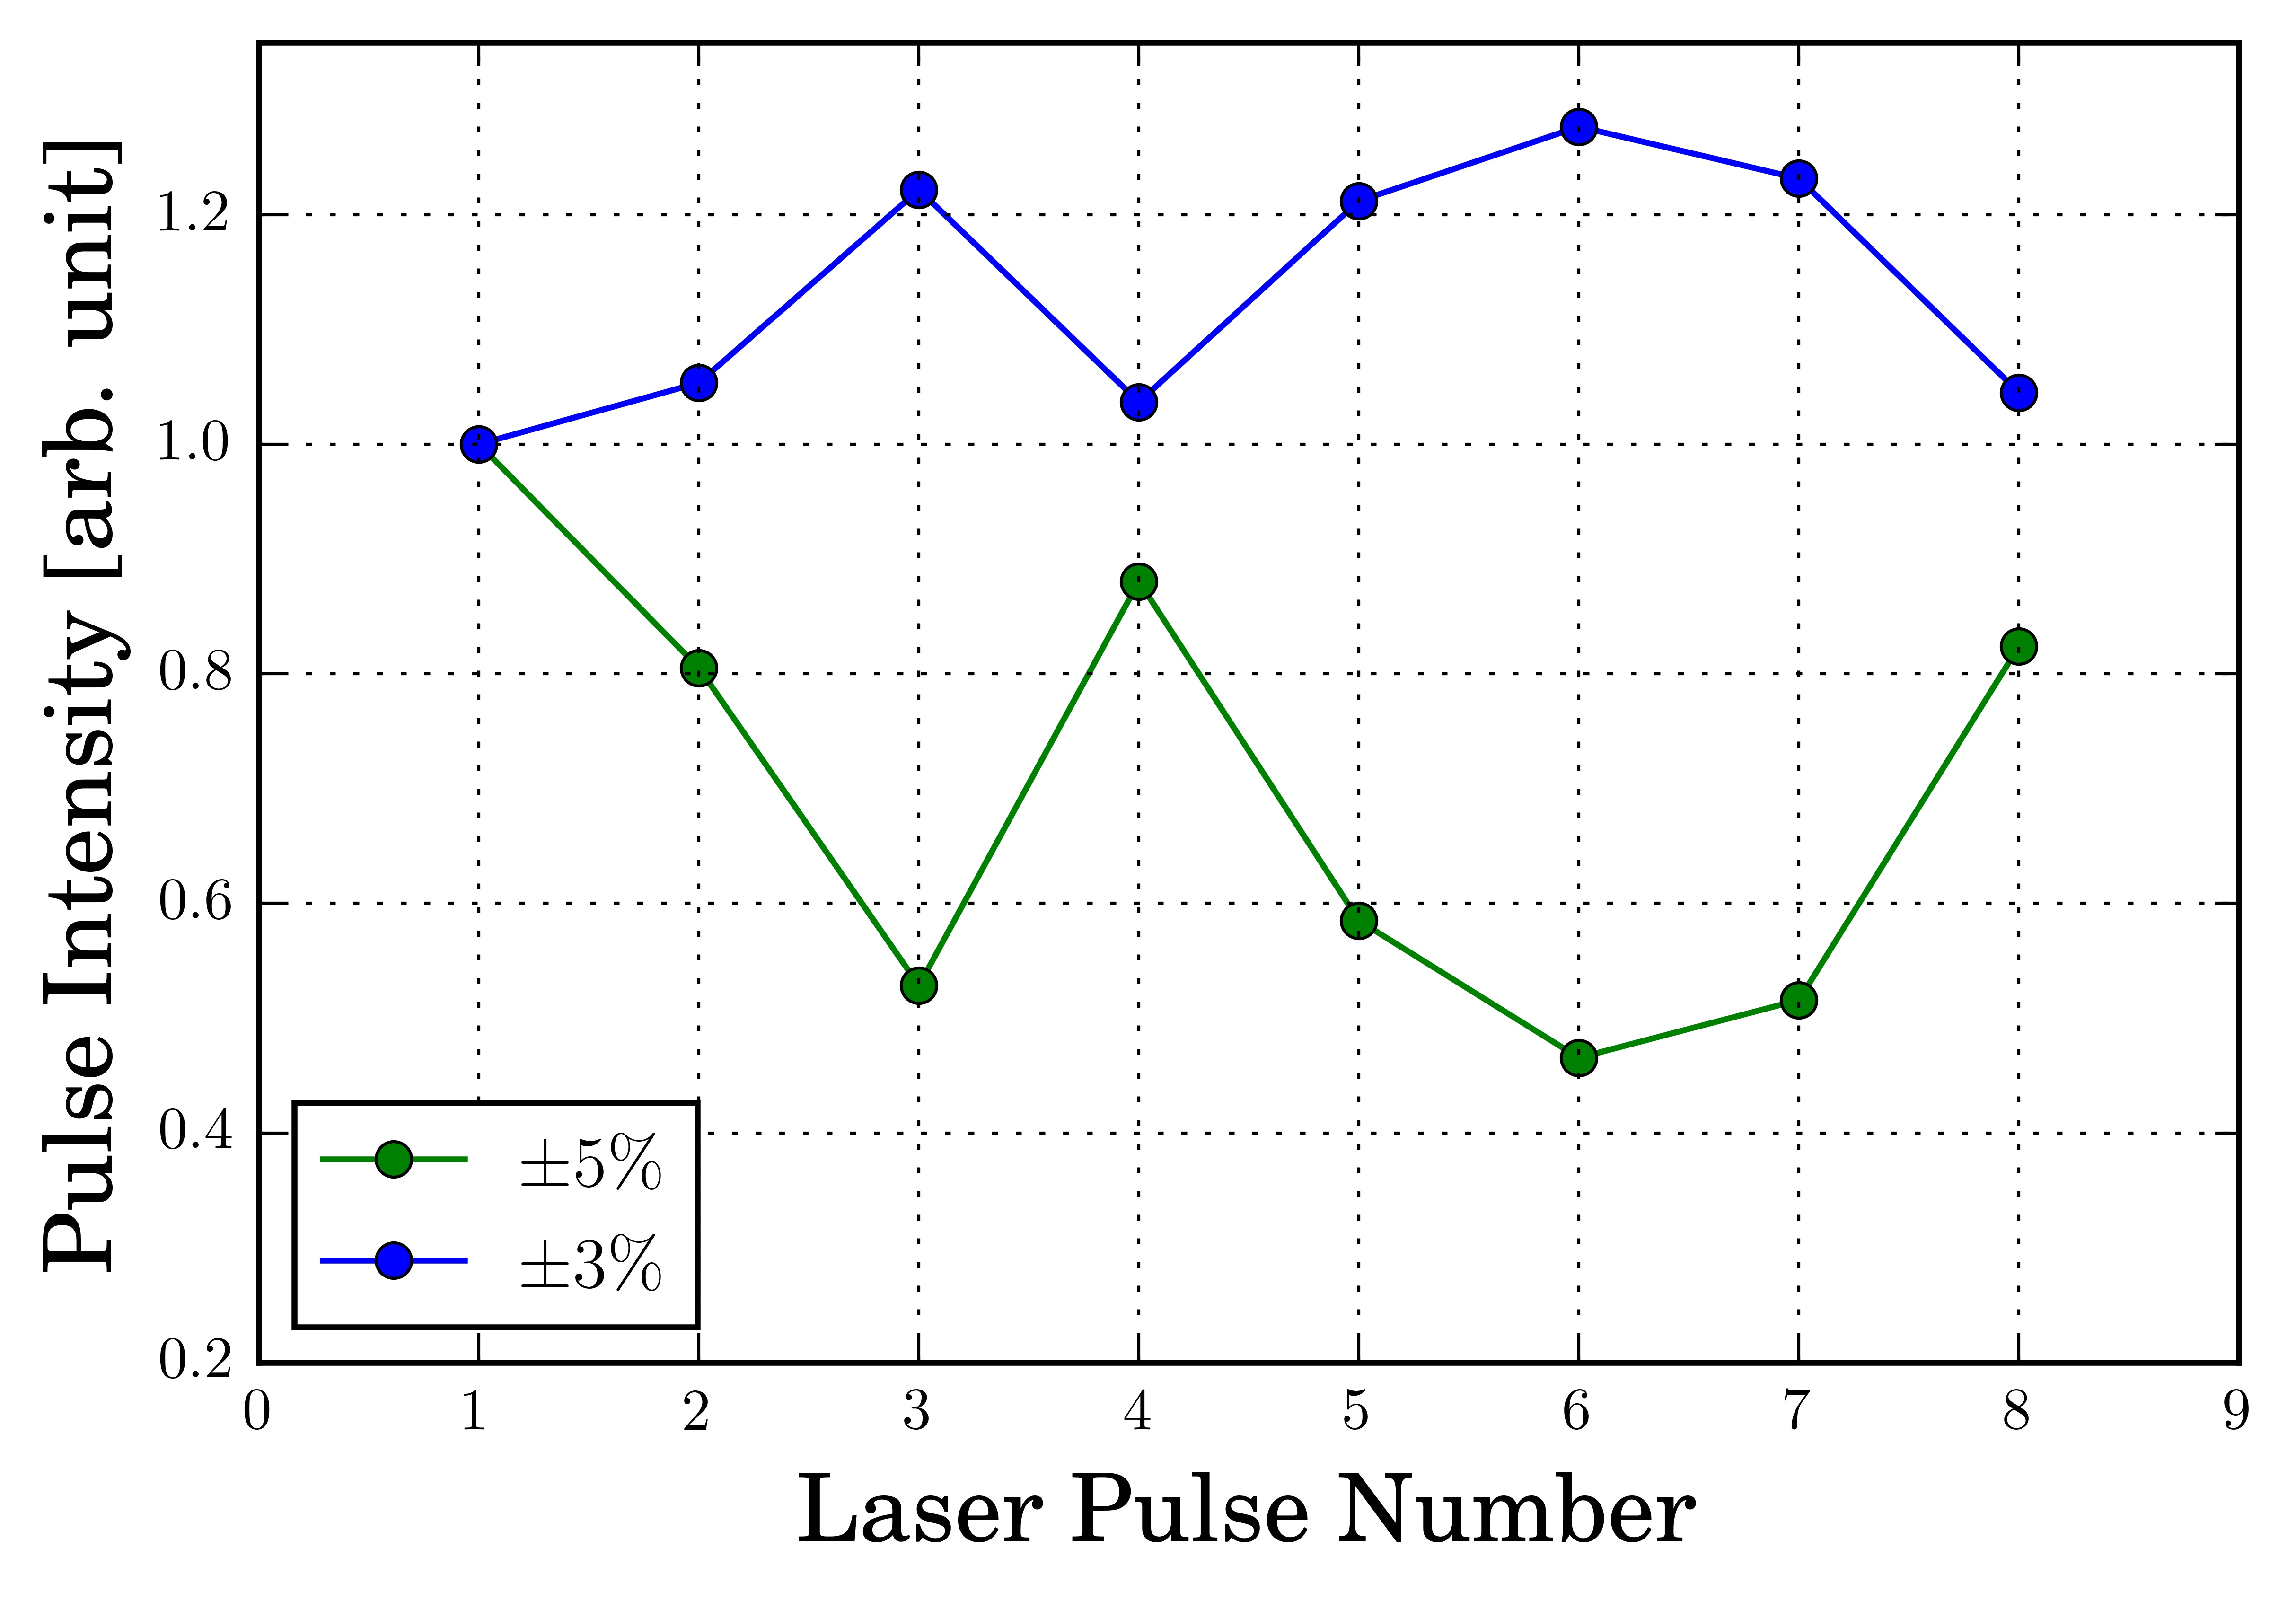
\includegraphics[width=0.8\textwidth]{images/splitter_improvement}\caption{Laser pulse train intensity measurements}
	\end{center}
	\label{fig:origtrain}
\end{figure}
\fi
The predictions in Eqs.~\ref{eq:i4} and~\ref{eq:i6} don't account for mirror losses in the delay legs, 
so we expect a lower value in experiment. To do a quick check on whether or not these results are 
expected, consider laser pulse one and only four splitters (as was the experimental set up). 
Laser pulse one has a similar path to laser pulse four (Eq.~\ref{eq:i4}). 

\begin{equation}
I_1 = R \cdot T \cdot T \cdot T \cdot I_0 
\end{equation}

Given about $\pm10\%$ mirror loss in the delay legs, we expect laser pulse one and four 
to be roughly the same intensity. This is shown in Fig.~\ref{fig:origtrain}. With the same 
logic, we expect pulse six to have the largest deviation from pulse one, as it is reflected 
three times and transmitted once in the four splitter set up. This expectation is also 
confirmed by the results in Fig.~\ref{fig:origtrain}.  \lsnote{You achieved a significant improvement in the uniformity of the laser pulse train, as can be seen in the figure.  Even though it can be seen in the figure, you should wrap up the section with a quantitative statement about the improvement you achieved, along with a summary sentence on how you achieved it.  Something like, `Through the use of optics with tighter specifications, and sorting of the optical elements, an improvement in laser pulse uniformity of bla percent was achieved.'}  

%%%%%%%%%%%%%%%%%%%%%%%%%%%%%%%%%%%%%%%%%%%%%%%%%%%%%%%%%%%%%%%%%%%%%%%%%%%%%%%%%%%%%%%%%%%%
%%%%%%%%%%%%%%%%%%%%%%%%%%%%%%%%%%%%%%%%%%%%%%%%%%%%%%%%%%%%%%%%%%%%%%%%%%%%%%%%%%%%%%%%%%%%
\Section{RF Measurements}
%%%%%%%%%%%%%%%%%%%%%%%%%%%%%%%%%%%%%%%%%%%%%%%%%%%%%%%%%%%%%%%%%%%%%%%%%%%%%%%%%%%%%%%%%%%%
%%%%%%%%%%%%%%%%%%%%%%%%%%%%%%%%%%%%%%%%%%%%%%%%%%%%%%%%%%%%%%%%%%%%%%%%%%%%%%%%%%%%%%%%%%%%
In order to accurately simulate the RF fields in the cavities on the drive and witness line, 
a set of detailed measurements were done to determine the power in each RF cavity.
This includes power and energy measurements of the drive gun, and linac tanks 
one through 6 on the drive line.
\lsnote{You have a gun section below, so you should mention that in this paragraph as well as the cavities.}

\Subsection{Cable Calibration} \label{cablecal}
There is a significant length of cable that connects the cavities to the control room.
To calibrate these cables, a signal generator was placed in the tunnel. 
Then a signal was propagated to the control room where it was 
measured and compared to the original power measurement in the tunnel. 
\begin{figure*}[h]
	\begin{center}	
		\begin{circuitikz}[scale=0.7]
            \draw (0,0) to[csV=] (2,0);
            \node[align=center] at (0.8,1.5) {Signal \\ Generator};
            
			%Control room or power meter
			\def \leftside {3}
			\def \topbox {0.75}
			\def \botbox {-0.75}
			\draw (2.0, 0) -- (\leftside, 0);
			\draw[fill=white, ultra thick, rounded corners =0.1cm] (\leftside,\botbox)rectangle  
			({\leftside+3},\topbox) node[pos=0.5, align=center] {Meter};           
		\end{circuitikz}
    \end{center} 
\caption{Refrence power reading was taken while power meter was directly connected to the 
signal generator. The resulting power was $P_s=\SI{-8.92}{dBm}$}
\label{fig:signalgenerator}
\end{figure*}


\def \delayvertical {1.5}
\iftrue
\begin{figure*}[h]
	\begin{center}	
		\begin{circuitikz}[scale=0.7]
			
			\draw (0,0) to[csV=] (2,0);
			\node[align=center] at (0.8,1.5) {Signal \\ Generator};
			%Short blue RF cable 
			\node[] at (3.5,1) {$C_{1}$};
			\node[tlinestub] at (2,0){};
			\node[] at (3.5,-1) {};
			
			%Long RF cable
			\node[] at (7,1) {$C_{2}$};
			\node[tlinestub] at (5.5,0){};
			
			%Short yellow RF cable
			\node[] at (9.5,1) {$C_{3}$};
			\node[tlinestub] at (8.1,0){};
			\draw[] (4.6,0) to[short,-] ++(1,0);
			
			%10 dB attenuator
			\draw (10.7,0) to[R=$\SI{10}{dB}$, color=red] (14,0);
			
			%Control room or power meter
			\def \leftside {14}
			\def \topbox {0.75}
			\def \botbox {-0.75}
			%\draw (10.75, 0) -- (\leftside, 0);
			\draw[fill=white, ultra thick, rounded corners =0.1cm] (\leftside,\botbox)rectangle  
			({\leftside+3},\topbox) node[pos=0.5, align=center] {Meter};
		\end{circuitikz}
	\end{center} 
	\caption{Experimental set up when calibrating the cables from gun to control room. 
		Where $C_1$ is a short blue heliax, $C_2$ is a long heliax to the control room, 
		and $C_3$ is a short yellow heliax to the 6 GHz scope or power meter.}
	\label{fig:tikzcalibration}
\end{figure*}
\fi
The power reading in the control room was $P_c = \SI{-9.48}{dBm}$, and the power reading in 
the tunnel from the signal generator was $P_s = \SI{-8.92}{dBm}$, so the
attenuation is $\SI{0.56}{dB}$. However, one more cable needs to be accounted for and 
subtracted from the overall attenuation. A short blue heliax was used to connect the 
signal generator to the control room cables, as shown in Fig.~\ref{fig:tikzcalibration}.
This cable not normally connected to the control room as shown in Fig.~\ref{fig:tikzdrivegun}. \lsnote{You should finish the thought - how much attenuation from the Heliax, and what is the adjusted correction?}


\Subsection{Drive Gun Measurements}
After the cable calibration, the set up was returned to typical rf conditions as 
shown in Fig.~\ref{fig:tikzdrivegun}. This includes $\SI{53.2}{dB}$ from the pick 
up probe itself, a $\SI{36}{dB}$ additional attenuation connected to the 
drive gun pick up probe, followed by a long heliax to the 
control room. The signal split in the control room with a mini-circuit ZX10-2-12+. 
One port is used for Low Level RF (LLRF) control, and the other port was connected to a short 
heliax, $C_3$, then to a $\SI{10}{dB}$ attenuator and finally to the 
power meter. Normally a load is placed at port two when no power meter is connected. 
Next, the klystrons and phase shifters were set to supply 
max power to the gun, typical of TBA running conditions. 
\def \delayvertical {1.5}
\iftrue
\begin{figure*}[h]
	\begin{center}		
		\begin{circuitikz}[scale=0.7]
			\def \leftside {17.0}
			\def \topbox {0.75}
			\def \botbox {-0.75}
			
			\node[] at (0.8,1.3) {Gun};
			\draw (0,0) to[csV=] (2,0);
			
			\def \gunright {2}
			%Attenuators
			%\node at (2, -0.50) {$P_1$};
			%\node at (5, -0.50) {$P_2$};
			
			\draw (\gunright,0) to[R=$\SI{53.2}{dB}$, color=red] (\gunright+2,0);
			\draw (\gunright+2.5,0) to[R=$\SI{36}{dB}$, color=red] (\gunright+4.5,0);
			\draw[] (\gunright+2.0,0) to[short,-] ++(0.5,0);
			%Long RF cable
			
			\node[] at (\gunright+6,1) {$C_{2}$};
			\node[tlinestub] at (\gunright+4.5,0){};
			\draw (9.0, 0) -- (10.0, 0);
			\draw[fill=white, ultra thick, rounded corners =0.1cm] (\gunright+8.0,\botbox)rectangle  
			%splitter
			({\gunright+11.0},\topbox) node[pos=0.5, align=center] {Splitter};
			\draw (11.5, 0.7) -- (11.5, 2);
			\node[] at (11.5, 2.5) {LLRF};
			
			%Short yellow RF cable
			\draw (13.0, 0) -- (13.5, 0);
			\node[] at (\gunright+13.0,1) {$C_{3}$};
			\node[tlinestub] at (\gunright+11.5,0){};
						
			%10 dB attenuator
			\draw (16.0, 0) -- (16.5, 0);
			\draw (\gunright+14.5,0) to[R=$\SI{10}{dB}$, color=red] (\gunright+16.5,0);
			
			%Control room or power meter
			\draw (18.5, 0) -- (\leftside+2, 0);
			\draw[fill=white, ultra thick, rounded corners =0.1cm] (\leftside+2,\botbox)rectangle  
			({\leftside+5},\topbox) node[pos=0.5, align=center] {Meter};
		\end{circuitikz}
	\end{center} 
	\caption{Experimental set up when measuring power from gun to control room. 
		Where $\SI{53.2}{dB}$ of attenuation is due to the gun probe itself, 
		$\SI{36}{dB}$ of additional attenuation is attached to gun pick up probe cable in the tunnel, 
		$C_2$ is a long heliax to the control room. The $\SI{10}{dB}$  splitter sends half the signal to the   
		low level RF (LLRF) control system, and half to the power meter. 
		$C_3$ is a short yellow heliax that connects the meter to the splitter and on to the 6 GHz scope or power meter.}
	\label{fig:tikzdrivegun}
\end{figure*}
\fi

Using the set up in Fig.~\ref{fig:tikzdrivegun}, the power meter measured  $P_{g} = \SI{-14.18}{dBm}$
in the control room. Now we must account for attenuation to know the true power
signal out of the gun. 
\begin{equation}
P_g \, \SI{}{[dBm]} = \SI{53.2}{dB} + \SI{36}{dB} + \SI{0.56}{dB} + \SI{10}{dB}+ \SI{10}{dB} - \SI{14.18}{dBm} = \SI{95.58}{dBm}
\end{equation}

Then converting to a more convenient unit: 
\begin{equation}
P \, \SI{}{[dBm]} = 10 \cdot \log{\frac{P \, \SI{}{[mW]}}{\SI{1}{[mW]}}}
\end{equation}
\begin{equation} \label{eq:dbmtomw}
P \, \SI{}{[mW]} = \SI{1}{[mW]} \cdot 10^{\frac{P \, [\SI{}{dBm}]}{\SI{10}{}}}
\end{equation}
\begin{equation} 
P_2 = 10^{\SI{9.56}{dBm}} \cdot  \SI{1}{[mW]} = 3.6 \, \SI{}{[MW]} 
\end{equation}

\Subsection{Linac Cavity Measurements}
There are six linear accelerating (linac) cavities after the gun. 
Each are connected to the control room in the same way as the gun. 
The only differences are in the attenuation at the pick up probe and 
the splitter attenuation. The power readings for each tank are: 
$L_i=[-18.9,-12.2,-18.9,-17.8,-14.3]\pm \SI{0.05}{dBm}$. 

\begin{equation}
P_1 = \SI{0}{dB} + \SI{0}{dB} + \SI{0.56}{dB} + 
\end{equation}



%%%%%%%%%%%%%%%%%%%%%%%%%%%%%%%%%%%%%%%%%%%%%%%%%%%%%%%%%%%%%%%%%%%%%%%%%%%%%%%%%%%%%%%%%%%%
%%%%%%%%%%%%%%%%%%%%%%%%%%%%%%%%%%%%%%%%%%%%%%%%%%%%%%%%%%%%%%%%%%%%%%%%%%%%%%%%%%%%%%%%%%%%
\Section{Energy Measurements} \label{sec:dipolecal}
%%%%%%%%%%%%%%%%%%%%%%%%%%%%%%%%%%%%%%%%%%%%%%%%%%%%%%%%%%%%%%%%%%%%%%%%%%%%%%%%%%%%%%%%%%%%
%%%%%%%%%%%%%%%%%%%%%%%%%%%%%%%%%%%%%%%%%%%%%%%%%%%%%%%%%%%%%%%%%%%%%%%%%%%%%%%%%%%%%%%%%%%%
Energy measurements at the AWA are done with a traditional 
spectrometer. This includes a dipole magnet and two Yittrium 
Aluminum Garnet (YAG) screens as shown in Fig~\ref{fig:spectrometer}.

\begin{figure*}[h]
	\begin{center}		
		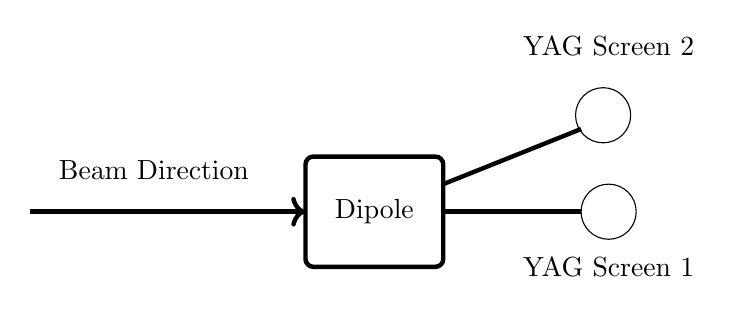
\begin{tikzpicture}[scale=0.7]
			
			\node[] at (2.25,0.75) {Beam Direction};
			\draw[ultra thick, ->] (0,0) -- (5.0, 0.0);
			
			\draw[fill=white, ultra thick, rounded corners =0.1cm] (5.0,1.0)rectangle  
			(7.5,-1.0) node[pos=0.5, align=center] {Dipole};
			
			\draw[ultra thick] (7.5, 0.0) -- (10.0, 0.0);
			\draw[ultra thick] (7.5, 0.5) -- (10.0, 1.5);
						
			\node[] at (10.5, 3) {YAG Screen 2};
			\draw (10.4,1.75) circle (0.5cm);
			
			\node[] at (10.5, -1.0) {YAG Screen 1};
			\draw (10.5,0) circle (0.5cm);
			
		\end{tikzpicture}
	\end{center} 
	\caption{Spectrometer set up in all cases at AWA.}
	\label{fig:spectrometer}
\end{figure*}

\Subsection{Energy Measurement Procedure}
Taking an energy measurement requires a beam trajectory
that is centered through the dipole. Otherwise, the beam 
may experience excessive non-uniform fields 
if it enters the dipole off-axis. The centering is done with two 
quads before the dipole. The center is found by focusing 
in the x-direction, and then the y-direction. If the beam 
moves to the left or the right as it is being focused, 
the quad is "steering", and the beam is entering the magnets off-axis.
Once the beam is centered through the quads on YAG screen 1, 
the dipole is then turned on to bend the beam.
The two YAG screens are positioned so that when the dipole is off, 
a centered beam will hit YAG screen 1. When the dipole is turned
on, the beam will appear at the center of YAG screen 2 when the 
beam is bent $20^\circ$. In this way, the dipole strength can 
then be used to determine the beam energy.

\Subsection{Energy Calculation}
Based on the procedure above, there is one number which we 
use to back calculate the mean energy. The amount of current
supplied to the dipole is represented by the number of "counts"
keyed into the control system. A counts to current line
is calculated given the measurements shown in Table \ref{tab:counts}
\begin{table}
\begin{center}
	\begin{tabular}{||c c||} 
		\hline
		Counts & Current [A] \\ [0.5ex] 
		\hline\hline
		1000 & 3.7 \\ 
		\hline
		5000 & 18.8 \\
		\hline
		10000 & 37.5 \\
		\hline
		15000 & 56.3 \\
		\hline
		
	\end{tabular}
\end{center}
\caption{Counts to current data for the first dipole in the drive beam line.}
\end{table}\label{tab:counts}
Then the B-field is calculated given the current: 
\begin{equation}
	\SI{}{B\,[T]} = (180.9708\cdot \SI{}{I\,[A]} - 7.2053)\cdot 10^{-4}
\end{equation}
There are a few geometric calculations that need to be done using the magnetic field value. 
before we can calculate the energy. 
The radius of curvature, $\rho$, 
can be calculated using the effective length of the dipole, L, and bending angle, $\theta$.
\begin{equation}
	\rho = \frac{L}{2\cdot \sin(\frac{\theta}{2})}
\end{equation}
Using $\rho$, and geometry, we can also estimate the x offset of the
beam after the dipole: 
\begin{equation}
	\Delta x = \rho \left( 1- \cos\theta \right)
\end{equation}
Using this and the famous relationship, $B\rho$ \cite{Wiedemann},
we can relate the B field and the beam momentum. 
\begin{equation}
	\SI{}{p\,\left[\frac{MeV}{c}\right]} = \frac{B\cdot \rho}{3.3356}\cdot 10^3
\end{equation}
We can then calculate the total energy by including the rest mass of the electrons \cite{Griffiths}:
\begin{equation}
	\SI{}{E\,[MeV]} = \sqrt{0.511^2+p^2}
\end{equation}\label{eq:energy}

\Subsubsection{Hard Edge Dipole Example}
\nrnote{this example is more of a double check and reference for me than for the reader...}
Since this calculation is used several time throughout the 
beam line for different magnets, lets consider a hard edge 
dipole, to show how the above equations can be used to determine
the x offset after the magnet, and the beam energy. 

Let's define the dipole length, $L=\SI{0.2}{[m]}$, angle, $\theta=\SI{20}{degrees}$. 
The corresponding radius is $\rho = \SI{0.5759}{[m]}$. With these values we can now 
calculate the offset, $\Delta x \approx \SI{34}{[mm]}$, which is confirmed by OPAL. 

\nrnote{not sure if I want to include energy since it depends on measured counts....}
Given a count of  energy of $\SI{64.8}{[MeV]}$ given measured counts of 

%%%%%%%%%%%%%%%%%%%%%%%%%%%%%%%%%%%%%%%%%%%%%%%%%%%%%%%%%%%%%%%%%%%%%%%%%%%%%%%%%%%%%%%%%%%%
%%%%%%%%%%%%%%%%%%%%%%%%%%%%%%%%%%%%%%%%%%%%%%%%%%%%%%%%%%%%%%%%%%%%%%%%%%%%%%%%%%%%%%%%%%%%
\Section{Transverse Beam Size Measurements} \label{sec:beamsize}
%%%%%%%%%%%%%%%%%%%%%%%%%%%%%%%%%%%%%%%%%%%%%%%%%%%%%%%%%%%%%%%%%%%%%%%%%%%%%%%%%%%%%%%%%%%%
%%%%%%%%%%%%%%%%%%%%%%%%%%%%%%%%%%%%%%%%%%%%%%%%%%%%%%%%%%%%%%%%%%%%%%%%%%%%%%%%%%%%%%%%%%%%
Beam size measurements are taken by using YAG screens at multiple z locations along the beam line.
The code used to produce all the following images can be found at this git repository:

\url{https://github.com/nneveu/imageProcessing}

\Subsection{Capturing Images}
\nrnote{Add tikz picture here to show how camera is pointed into beam line with mirrors}

\Subsection{Post Processing Images}
A python script was written to take beam images and convert them to profiles in the x and y direction.
This is done in a series of steps, and requires that one or more images can be used as a 
background image and fiducial image. A background image must capture any dark current 
that is present when the beam is not hitting the YAG screen. The fiducial image must 
clearly show the edges of the YAG screen so that a mm/pixel conversion can be calculated.
The following steps detail the post processing from raw image to transverse beam size estimate.

\subsubsection{Step 1: Calculating the fiducial}

\subsubsection{Step 2: Remove background intensity}

\subsubsection{Step 3: Calculate x and y beam profile}

\subsubsection{Step 4: Fit profile to calculate beam size}




%\Subsection{Kicker }
%%%%%%%%%%%%%%%%%%%%%%%%%%%%%%%%%%%%%%%%%%%%%%%%%%%%%%%%%%%%%%%%%%%%%%%%%%%%%%%%%%%%%%%%%%%%
%%%%%%%%%%%%%%%%%%%%%%%%%%%%%%%%%%%%%%%%%%%%%%%%%%%%%%%%%%%%%%%%%%%%%%%%%%%%%%%%%%%%%%%%%%%%
%\SubSection{Septum } 
%%%%%%%%%%%%%%%%%%%%%%%%%%%%%%%%%%%%%%%%%%%%%%%%%%%%%%%%%%%%%%%%%%%%%%%%%%%%%%%%%%%%%%%%%%%%
%%%%%%%%%%%%%%%%%%%%%%%%%%%%%%%%%%%%%%%%%%%%%%%%%%%%%%%%%%%%%%%%%%%%%%%%%%%%%%%%%%%%%%%%%%%%
\Chapter{Beam Dynamics}  
%%%%%%%%%%%%%%%%%%%%%%%%%%%%%%%%%%%%%%%%%%%%%%%%%%%%%%%%%%%%%%%%%%%%%%%%%%%%%%%%%%%%%%%%%%%%
%%%%%%%%%%%%%%%%%%%%%%%%%%%%%%%%%%%%%%%%%%%%%%%%%%%%%%%%%%%%%%%%%%%%%%%%%%%%%%%%%%%%%%%%%%%%
\Section{Code and Resources Used}\label{sec:code}
%%%%%%%%%%%%%%%%%%%%%%%%%%%%%%%%%%%%%%%%%%%%%%%%%%%%%%%%%%%%%%%%%%%%%%%%%%%%%%%%%%%%%%%%%%%%
%%%%%%%%%%%%%%%%%%%%%%%%%%%%%%%%%%%%%%%%%%%%%%%%%%%%%%%%%%%%%%%%%%%%%%%%%%%%%%%%%%%%%%%%%%%%

\lsnote{You need to start the chapter with summary paragraphs.  (1) Why are simulations needed?  (2) What simulation work was done?  (3) What method was chosen and why?  (4) What were the results?  You can't put  all of that in now, since some of it is unknown, but you should do (1), (3) and part of (2).  Also, before launching into the OPAL stuff, you need to say a few words about the beam characteristics during TBA studies.  A table of beam characteristics would be good here, one for the drive beam, and one for the witness.  After presenting the beam characteristics, you can mention that space charge is a problem for the drive beam - since now they know the intensity.}

To simulate beam dynamics, the particle-in-cell (PIC) code OPAL was used \cite{opal}. PIC codes simulate 
the electromagnetic forces that particles see in an accelerator. This is done by mapping the input 
particles onto a grid. Then in each time (or z) step, the forces due to space charge, accelerating gradients, 
and magnets are calculated and applied to the grid. 
\lsnote{You need a few sentences describing OPAL.  Also describe (briefly) what a PIC code is.  (Are there any other choices besides a PIC code?)}
It was chosen for several reasons:
\begin{itemize}
	\item Able to calculate transverse space charge and wakefield forces 
	\item Option to run the code in parallel
	\item Data recorded in global and reference frames
\end{itemize} 

The first item is crucial to standard operations at the AWA. Especially in the 
case of TBA, high charge is needed on drive beam line, therefore transverse 
space charge must be calculated in the simulations to give realistic results.

The second item dramatically reduced the amount of simulation time needed. 
Typical running conditions were on 16 cores, and for random samples up to 128 cores.  \lsnote{Specifics are always good; do you have any numbers for the time for a parallel run versus single processor?  If not, it is not super important, but if those numbers are handy put them in.}

%%%%%%%%%%%%%%%%%%%%%%%%%%%%%%%%%%%%%%%%%%%%%%%%%%%%%%%%%%%%%%%%%%%%%%%%%%%%%%%%%%%%%%%%%%%%
%%%%%%%%%%%%%%%%%%%%%%%%%%%%%%%%%%%%%%%%%%%%%%%%%%%%%%%%%%%%%%%%%%%%%%%%%%%%%%%%%%%%%%%%%%%%
\Section{Optimization Techniques} \label{sec:opt}
%%%%%%%%%%%%%%%%%%%%%%%%%%%%%%%%%%%%%%%%%%%%%%%%%%%%%%%%%%%%%%%%%%%%%%%%%%%%%%%%%%%%%%%%%%%%
%%%%%%%%%%%%%%%%%%%%%%%%%%%%%%%%%%%%%%%%%%%%%%%%%%%%%%%%%%%%%%%%%%%%%%%%%%%%%%%%%%%%%%%%%%%%
\Section{Simulation Results} \label{sec:simulations}
%%%%%%%%%%%%%%%%%%%%%%%%%%%%%%%%%%%%%%%%%%%%%%%%%%%%%%%%%%%%%%%%%%%%%%%%%%%%%%%%%%%%%%%%%%%%
%%%%%%%%%%%%%%%%%%%%%%%%%%%%%%%%%%%%%%%%%%%%%%%%%%%%%%%%%%%%%%%%%%%%%%%%%%%%%%%%%%%%%%%%%%%%
Simulations were done for both the drive and witness beam line. 
This included both photoinjectors, linacs, and wakefield effects. 

\Subsection{Benchmarking: Gun Simulations}
\nrnote{Add benchmark here}
At 40nC the usable gun phase range (for the 3D field map) is 
$-30^\circ \le \phi_g \ge 30^\circ$. The usable region was defined 
as the region where all particles are emitted from the gun. 
i.e. at $40^\circ$, particles were lost.  

\Subsection{Linac Simulations and Pareto Front} \label{sec:pareto}

In order to optimize the beam entering the TBA experimental area, 
simulations were done to minimize the emittance after the 6 cavity linac
on the drive side. 
%%%%%%%%%%%%%%%%%%%%%%%%%%%%%%%%%%%%%%%%%%%%%%%%%%%%%%%%%%%%%%%%%%%%%%%%%%%%%%%%%%%%%%%%%%%%
%%%%%%%%%%%%%%%%%%%%%%%%%%%%%%%%%%%%%%%%%%%%%%%%%%%%%%%%%%%%%%%%%%%%%%%%%%%%%%%%%%%%%%%%%%%%
%\Section{Kicker}




%%%%%%%%%%%%%%%%%%%%%%%%%%%%%%%%%%%%%%%%%%%%%%%%%%%%%%%%%%%%%%%%%%%%%%%%%%%%%%%%%%%%%%%%%%%%
%%%%%%%%%%%%%%%%%%%%%%%%%%%%%%%%%%%%%%%%%%%%%%%%%%%%%%%%%%%%%%%%%%%%%%%%%%%%%%%%%%%%%%%%%%%%
\Subsection{Kicker Design}

\lsnote{You need to start with a re-statement of the purpose of the kicker. }
A design implemented by Indiana University (IU) \cite{iukicker}
will be adapted to fit TBA requirements at the AWA. Redesign will require optimization
of the length and gap between the kicker plates. \lsnote{Summarize what criteria are used to determine these.} Figure \ref{fig:IUkicker} shows the existing IU kicker.
\begin{figure}[h]
	\begin{center}
		%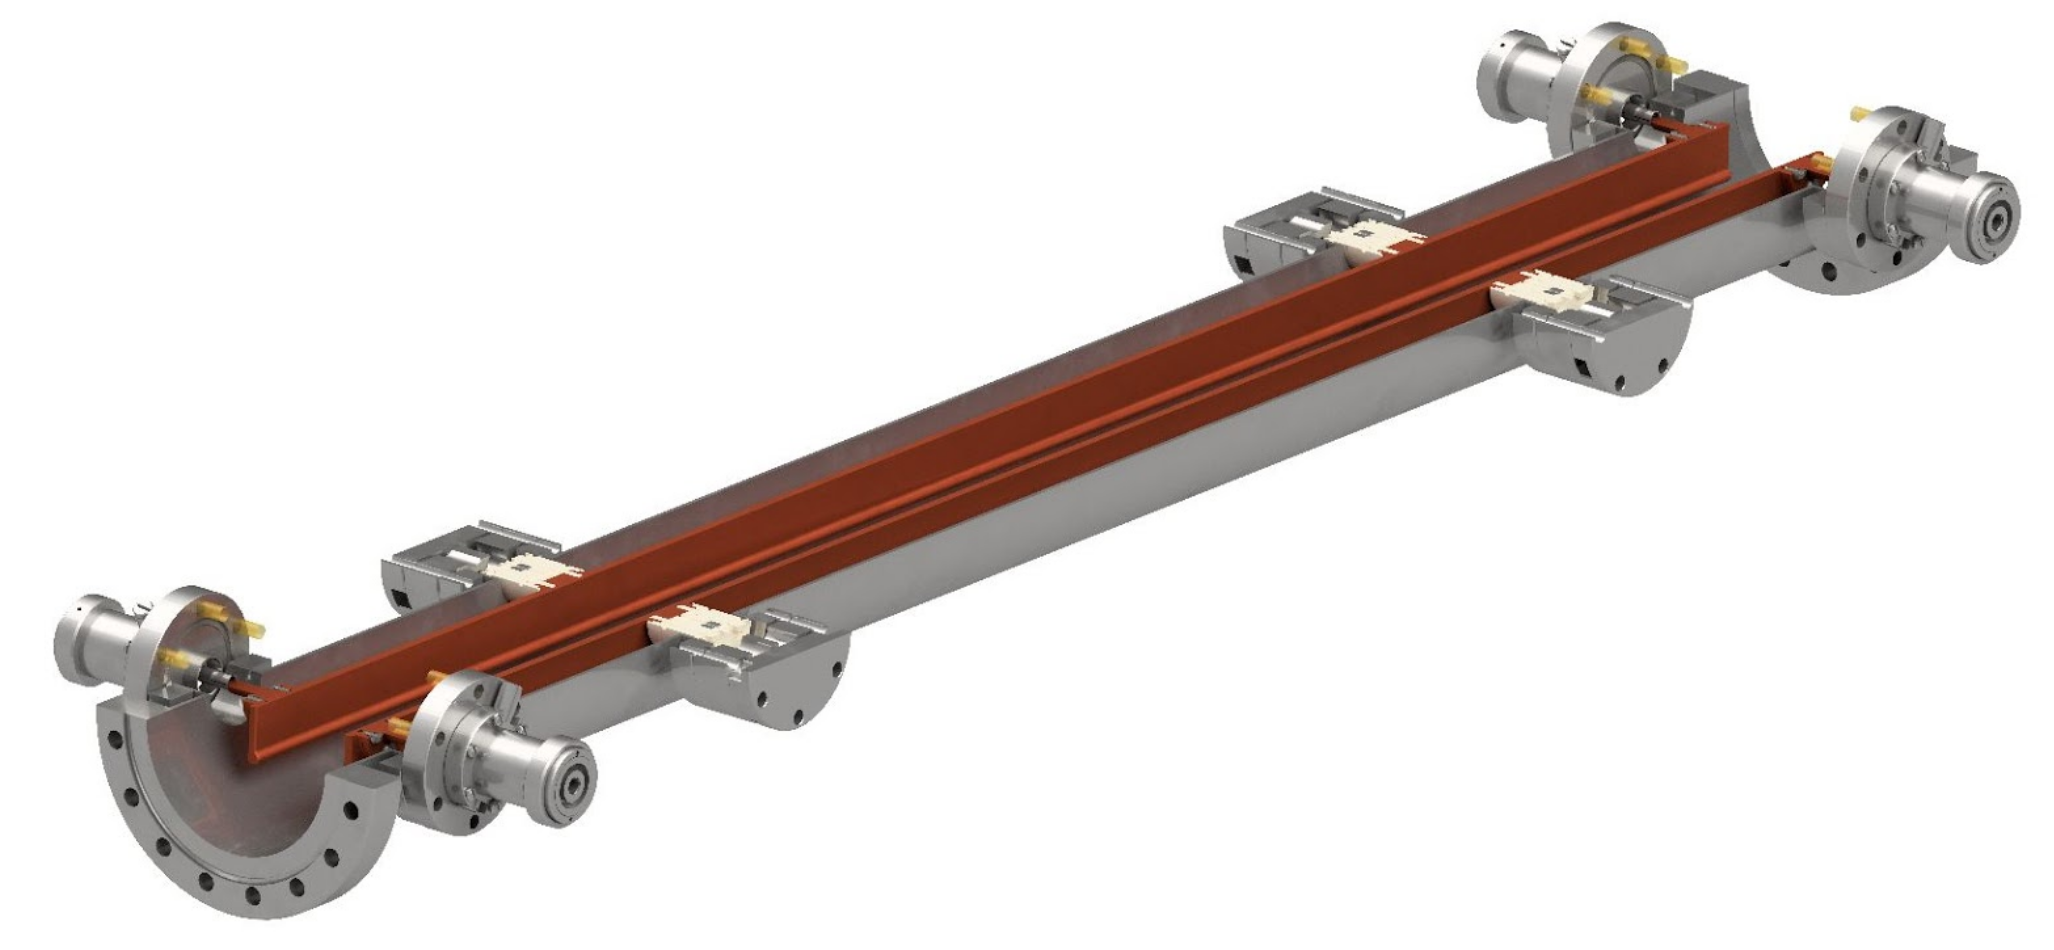
\includegraphics[scale=0.5]{C:/Users/nneveu/Pictures/kicker.jpg}\caption{IU Kicker \cite{IUkicker}}
		\label{fig:IUkicker}
	\end{center}
\end{figure}
The kicker is essentially a parallel plate waveguide. 
A $\pm$35 kV power supply will be used to induce a 70 kV potential difference 
across the plates. Each plate will be terminated in a 50 $\Omega$ load to induce a steady 
state current on the plates. The combination of the two will result in a static TEM mode 
between the plates. Calculation of the electric, $E_v$, and magnetic field, $B_v$,
can be derived from the voltage or current. The electric field, $E_v$, due to a potential, V, is: 
\begin{equation}
E_v=\frac{V}{h}
\end{equation}

Where h is the gap height. From Maxwell's equations, we know that the electric and magnetic 
field are related by the speed of light, c, in the case of plane and TEM waves \cite{pozar}. 
From this we can find the magnetic field induced between the plates: 
\begin{equation}
B_v=\frac{E_v}{c}
\end{equation}
The electrons are going at the speed of light, $c$, and are moving through the kicker on a 
trajectory perpendicular to the fields.  So, it can be seen from the Lorentz force equation, that the force 
exerted on a charge q from the electric and magnetic fields of the TEM mode are equal. 
\begin{equation}
F=q(E_v+v\times B_v)
\end{equation}

Since the force due to the electric field is equal and in the same direction as that from the magnetic field, 
the total kick is just twice that from either field alone.  The angle induced by each field is \cite{iukicker, Wiedemann}:  
\begin{equation}
\theta_E= \frac{V\,L}{h\,T}
\end{equation}
\begin{equation}
\theta_B= \frac{B\,L}{B\rho}
\end{equation}

Where L is the plate length, and T is the kinetic energy of the beam. $B\rho=3.33564\,*T\,$ [GeV-Tesla] is a 
common accelerator physics term that can be found in text such as Wiedemann \cite{Wiedemann}. 
The total angle provided by the kicker is then: 
\begin{equation}
\theta_{total}= \theta_E+\theta_B=2\theta_E=2\theta_B
\end{equation}
From these equations, variable parameters include the gap height, length of the plates, and 
the kinetic energy of the beam. The largest drive beam energy achievable at the AWA is 75 MeV. 
Thesis work will include the optimization of these parameters to obtain the largest angle possible.
Simulations have begun to set boundary conditions on the variable parameters. 



\Chapter{Experimental Measurements}%________________________________

\Chapter{Experimental Results} 
%%%%%%%%%%%%%%%%%%%%%%%%%%%%%%%%%%%%%%%%%%%%%%%%%%%%%%%%%%%%%%%%%%%%%%%%%%%%%%%%%%%%%%%%%%%%
%%%%%%%%%%%%%%%%%%%%%%%%%%%%%%%%%%%%%%%%%%%%%%%%%%%%%%%%%%%%%%%%%%%%%%%%%%%%%%%%%%%%%%%%%%%%
\Section{Measurement of Single Stage Power Extraction}
%%%%%%%%%%%%%%%%%%%%%%%%%%%%%%%%%%%%%%%%%%%%%%%%%%%%%%%%%%%%%%%%%%%%%%%%%%%%%%%%%%%%%%%%%%%%
%%%%%%%%%%%%%%%%%%%%%%%%%%%%%%%%%%%%%%%%%%%%%%%%%%%%%%%%%%%%%%%%%%%%%%%%%%%%%%%%%%%%%%%%%%%%
%\Section{Measurement of Single Stage Accelerating Gradient}
%\Section{Measurement of Staged Two Beam Acceleration}

\footnote{My Footnote} 
\Chapter{CONCLUSION}
%   \input{Conclusion.tex}
You need a Conclusion.tex file

\Section{Summary}


This was just to create a sample section...

\clearpage


%
% APPENDIX
%
\appendix

\Appendix{Calculations?}

......

%\moretox

\Appendix{OPAL stuff? MCS Stuff?}

Your second appendix text....

\newpage
%
% BIBLIOGRAPHY
%
\bibliographystyle{plain}
\bibliography{thesis}

\end{document}  % end of document





























